\newpage\handout
{Drill Problems: Week 3.1}
{\textsc{Scholastic Aptitude Test (SAT)}}
{\href{https://creativecommons.org/licenses/by-nc-sa/4.0/}{CC BY-NC-SA 4.0 license}}
{Author: \BookAuthor}{Release: \generatedOn}
{SAT: Drill Problems (3.1)}
% Copyright & Disclaimer
\begin{center}
  \begin{minipage}{0.85\textwidth}
    {\small\textbf{Purpose and Usage:}}\\[0.2cm]
    {\footnotesize
    This material has been developed for internal training and educational 
    purposes at Hans edu LLC. It is intended for use within our organization 
    and should not be distributed, sold, or used for commercial purposes 
    outside of our educational programs.}\\[0.5cm]
    
    {\small\textbf{For Our Community:}}\\[0.2cm]
    {\footnotesize
    Students and staff are welcome to use this material in their studies and 
    teaching at Hans edu LLC. While we encourage active engagement with the 
    content, please respect that this is proprietary material. Any 
    reproduction or distribution outside of our organization's educational 
    activities is not permitted.}\\[0.5cm]
    
    {\small\textbf{Content and Attribution:}}\\[0.2cm]
    {\footnotesize
    This material represents our adaptation of various established mathematics 
    textbooks, reorganized and enhanced for our teaching context. While we've 
    added our own pedagogical improvements, we maintain proper attribution to 
    original sources. This work is shared under the Creative Commons 
    Attribution-NonCommercial-ShareAlike (CC BY-NC-SA) license, allowing 
    internal use and adaptation while respecting the original creators' rights.
    % \small Key Permissions under CC BY-NC-SA 4.0:
    % \begin{itemize}
    %   \item credit the creator.
    %   \item no commercial use.
    %   \item new creations must carry the same license.
    %   \item copy and redistribute the material in any medium or format
    %   \item remix, transform, and build upon the material
    % \end{itemize}
    }\\[0.5cm]

    % Some content may be derived from sources under the CC0 1.0 Universal 
    % license, which allows for free use, modification, and distribution.}\\[0.5cm]
    {\small\textbf{Quality Assurance:}}\\[0.2cm]
    {\footnotesize
    We have carefully reviewed this material for accuracy and clarity. However, 
    as with any educational resource, we encourage critical engagement and 
    verification of concepts. If you notice any issues or have suggestions for 
    improvement, please bring them to our attention.}
  \end{minipage}
  
\includegraphics[width=0.45\textwidth]{images/CA_LastVersion.png}\\
  {\small © \the\year\ Hans edu LLC. All rights reserved.}\\[0.5cm]
  {\small Written by \BookAuthor}\\[1cm]
\end{center}

\newpage


\begin{enumerate}
  \item \textbf{Function Evaluation} (10 points)\\
  The function $g$ is defined by $g(x)=6x$. For what value of $x$ is $g(x)=54$?
  \begin{subanswer}
    % your answer here
  \end{subanswer}

  \item \textbf{Linear Function Definition} (10 points)\\
  In the $xy$-plane, the graph of the linear function $f$ contains the points $(0,3)$ and $(7,31)$. Which equation defines $f$, where $y=f(x)$?\\
  \begin{enumerate}[label=(\Alph*)]
    \item $f(x)=28x+34$
    \item $f(x)=3x+38$
    \item $f(x)=4x+3$
    \item $f(x)=7x+3$
  \end{enumerate}
  \begin{subanswer}
    % your answer here
  \end{subanswer}

  \item \textbf{Number Relationship} (10 points)\\
  The number $y$ is 84 less than the number $x$. Which equation represents the relationship between $x$ and $y$?\\
  \begin{enumerate}[label=(\Alph*)]
    \item $y=x+84$
    \item $y=\frac{1}{84}x$
    \item $y=84x$
    \item $y=x-84$
  \end{enumerate}
  \begin{subanswer}
    % your answer here
  \end{subanswer}

  \item \textbf{Function Value} (10 points)\\
  The function $f$ is defined by the equation $f(x)=7x+2$. What is the value of $f(x)$ when $x=4$?
  \begin{subanswer}
    % your answer here
  \end{subanswer}



  \newpage


  \item \textbf{Animal Weight Model} (10 points)\\
  A model predicts that a certain animal weighed 241 pounds when it was born and that the animal gained 3 pounds per day in its first year of life. This model is defined by an equation in the form $f(x)=a+bx$, where $f(x)$ is the predicted weight, in pounds, of the animal $x$ days after it was born, and $a$ and $b$ are constants. What is the value of $a$?
  \begin{subanswer}
    % your answer here
  \end{subanswer}

  \item \textbf{Function Evaluation} (10 points)\\
  The function $g$ is defined by $g(x)=-x+8$. What is the value of $g(0)$?\\
  \begin{enumerate}[label=(\Alph*)]
    \item -8
    \item 0
    \item 4
    \item 8
  \end{enumerate}
  \begin{subanswer}
    % your answer here
  \end{subanswer}

  \item \textbf{Function Value} (10 points)\\
  The function $f$ is defined by $f(x)=4x$. For what value of $x$ does $f(x)=8$?
  \begin{subanswer}
    % your answer here
  \end{subanswer}

  \newpage

  \item \textbf{Cab Ride Cost} (10 points)\\
  The line graphed in the $xy$-plane below models the total cost, in dollars, for a cab ride, $y$, in a certain city during nonpeak hours based on the number of miles traveled, $x$.

  \insertimage{0.40}{images/2025_06_15_1eff2981bb1cf12f04f1g-18}{reference attached}

  According to the graph, what is the cost for each additional mile traveled, in dollars, of a cab ride?\\
  \begin{enumerate}[label=(\Alph*)]
    \item \$2.00
    \item \$2.60
    \item \$3.00
    \item \$5.00
  \end{enumerate}
  \begin{subanswer}
    % your answer here
  \end{subanswer}

  \newpage

  \item \textbf{Cargo Movement} (10 points)\\
  A team of workers has been moving cargo off of a ship. The equation below models the approximate number of tons of cargo, $y$, that remains to be moved $x$ hours after the team started working.
  \[y=120-25x\]
  The graph of this equation in the $xy$-plane is a line. What is the best interpretation of the $x$-intercept in this context?\\
  \begin{enumerate}[label=(\Alph*)]
    \item The team will have moved all the cargo in about 4.8 hours.
    \item The team has been moving about 4.8 tons of cargo per hour.
    \item The team has been moving about 25 tons of cargo per hour.
    \item The team started with 120 tons of cargo to move.
  \end{enumerate}
  \begin{subanswer}
    % your answer here
  \end{subanswer}

  \newpage

  \item \textbf{Temperature Conversion} (10 points)\\
  \[F(x)=\frac{9}{5}(x-273.15)+32\]
  The function $F$ gives the temperature, in degrees Fahrenheit, that corresponds to a temperature of $x$ kelvins. If a temperature increased by 9.10 kelvins, by how much did the temperature increase, in degrees Fahrenheit?\\
  \begin{enumerate}[label=(\Alph*)]
    \item 16.38
    \item 48.38
    \item 475.29
    \item 507.29
  \end{enumerate}
  \begin{subanswer}
    % your answer here
  \end{subanswer}

  \item \textbf{Triangle Perimeter} (10 points)\\
  The perimeter of an isosceles triangle is 83 inches. Each of the two congruent sides of the triangle has a length of 24 inches. What is the length, in inches, of the third side?
  \begin{subanswer}
    % your answer here
  \end{subanswer}

  \item \textbf{Equation Solution} (10 points)\\
  $(b-2)x=8$\\
  In the given equation, $b$ is a constant. If the equation has no solution, what is the value of $b$?\\
  \begin{enumerate}[label=(\Alph*)]
    \item 2
    \item 4
    \item 6
    \item 10
  \end{enumerate}
  \begin{subanswer}
    % your answer here
  \end{subanswer}

  \item \textbf{Equation Solutions} (10 points)\\
  How many solutions does the equation $10(15x-9)=-15(6-10x)$ have?\\
  \begin{enumerate}[label=(\Alph*)]
    \item Exactly one
    \item Exactly two
    \item Infinitely many
    \item Zero
  \end{enumerate}
  \begin{subanswer}
    % your answer here
  \end{subanswer}

  \item \textbf{Equation Value} (10 points)\\
  $\frac{4x}{5}=20$\\
  In the equation above, what is the value of $x$?\\
  \begin{enumerate}[label=(\Alph*)]
    \item 25
    \item 24
    \item 16
    \item 15
  \end{enumerate}
  \begin{subanswer}
    % your answer here
  \end{subanswer}

  \item \textbf{No Solution Equation} (10 points)\\
  \[3(kx+13)=\frac{48}{17}x+36\]
  In the given equation, $k$ is a constant. The equation has no solution. What is the value of $k$?
  \begin{subanswer}
    % your answer here
  \end{subanswer}

  \item \textbf{Equivalent Equation} (10 points)\\
  Which of the following is equivalent to $4x+6=12$?\\
  \begin{enumerate}[label=(\Alph*)]
    \item $2x+4=6$
    \item $x+3=3$
    \item $3x+2=4$
    \item $2x+3=6$
  \end{enumerate}
  \begin{subanswer}
    % your answer here
  \end{subanswer}

  \item \textbf{Cost Calculation} (10 points)\\
  One pound of grapes costs \$2. At this rate, how many dollars will $c$ pounds of grapes cost?\\
  \begin{enumerate}[label=(\Alph*)]
    \item $2c$
    \item $2+c$
    \item $\frac{2}{c}$
    \item $\frac{c}{2}$
  \end{enumerate}
  \begin{subanswer}
    % your answer here
  \end{subanswer}

  \item \textbf{Flag Count} (10 points)\\
  A principal used a total of 25 flags that were either blue or yellow for field day. The principal used 20 blue flags. How many yellow flags were used?\\
  \begin{enumerate}[label=(\Alph*)]
    \item 5
    \item 20
    \item 25
    \item 30
  \end{enumerate}
  \begin{subanswer}
    % your answer here
  \end{subanswer}

  \item \textbf{Equation Solution} (10 points)\\
  \[8x=88\]
  What value of $x$ is the solution to the given equation?\\
  \begin{enumerate}[label=(\Alph*)]
    \item 11
    \item 80
    \item 96
    \item 704
  \end{enumerate}
  \begin{subanswer}
    % your answer here
  \end{subanswer}

  \item \textbf{Profit Calculation} (10 points)\\
  A certain product costs a company \$65 to make. The product is sold by a salesperson who earns a commission that is equal to 20\% of the sales price of the product. The profit the company makes for each unit is equal to the sales price minus the combined cost of making the product and the commission. If the sales price of the product is \$100, which of the following equations gives the number of units, $u$, of the product the company sold to make a profit of \$6,840?\\
  \begin{enumerate}[label=(\Alph*)]
    \item $(100(1-0.2)-65)u=6,840$
    \item $(100-65)(1-0.8)u=6,840$
    \item $0.8(100)-65u=6,840$
    \item $(0.2(100)+65)u=6,840$
  \end{enumerate}
  \begin{subanswer}
    % your answer here
  \end{subanswer}

  \item \textbf{Shipping Cost} (10 points)\\
  $3a+4b=25$\\
  A shipping company charged a customer \$25 to ship some small boxes and some large boxes. The equation above represents the relationship between $a$, the number of small boxes, and $b$, the number of large boxes, the customer had shipped. If the customer had 3 small boxes shipped, how many large boxes were shipped?\\
  \begin{enumerate}[label=(\Alph*)]
    \item 3
    \item 4
    \item 5
    \item 6
  \end{enumerate}
  \begin{subanswer}
    % your answer here
  \end{subanswer}

  \item \textbf{Parallel Line} (10 points)\\
  What is the equation of the line that passes through the point $(0,5)$ and is parallel to the graph of $y=7x+4$ in the $xy$ plane?\\
  \begin{enumerate}[label=(\Alph*)]
    \item $y=5x$
    \item $y=7x+5$
    \item $y=7x$
    \item $y=5x+7$
  \end{enumerate}
  \begin{subanswer}
    % your answer here
  \end{subanswer}

  \item \textbf{Time Relationship} (10 points)\\
  $$x+y=75$$
  The equation above relates the number of minutes, $x$, Maria spends running each day and the number of minutes, $y$, she spends biking each day. In the equation, what does the number 75 represent?\\
  \begin{enumerate}[label=(\Alph*)]
    \item The number of minutes spent running each day
    \item The number of minutes spent biking each day
    \item The total number of minutes spent running and biking each day
    \item The number of minutes spent biking for each minute spent running
  \end{enumerate}
  \begin{subanswer}
    % your answer here
  \end{subanswer}

  \newpage

  \item \textbf{Line Equation} (10 points)\\
  Line $t$ in the $xy$-plane has a slope of $-\frac{1}{3}$ and passes through the point $(9,10)$. Which equation defines line $t$?\\
  \begin{enumerate}[label=(\Alph*)]
    \item $y=13x-\frac{1}{3}$
    \item $y=9x+10$
    \item $y=-\frac{x}{3}+10$
    \item $y=-\frac{x}{3}+13$
  \end{enumerate}
  \begin{subanswer}
    % your answer here
  \end{subanswer}

  \item \textbf{Box Production} (10 points)\\
  A machine makes large boxes or small boxes, one at a time, for a total of 700 minutes each day. It takes the machine 10 minutes to make a large box or 5 minutes to make a small box. Which equation represents the possible number of large boxes, $x$, and small boxes, $y$, the machine can make each day?\\
  \begin{enumerate}[label=(\Alph*)]
    \item $5x+10y=700$
    \item $10x+5y=700$
    \item $(x+y)(10+5)=700$
    \item $(10+x)(5+y)=700$
  \end{enumerate}
  \begin{subanswer}
    % your answer here
  \end{subanswer}

  \item \textbf{Polygon Construction} (10 points)\\
  A total of 364 paper straws of equal length were used to construct two types of polygons: triangles and rectangles. The triangles and rectangles were constructed so that no two polygons had a common side. The equation $3x+4y=364$ represents this situation, where $x$ is the number of triangles constructed and $y$ is the number of rectangles constructed. What is the best interpretation of $(x,y)=(24,73)$ in this context?\\
  \begin{enumerate}[label=(\Alph*)]
    \item If 24 triangles were constructed, then 73 rectangles were constructed.
    \item If 24 triangles were constructed, then 73 paper straws were used.
    \item If 73 triangles were constructed, then 24 rectangles were constructed.
    \item If 73 triangles were constructed, then 24 paper straws were used.
  \end{enumerate}
  \begin{subanswer}
    % your answer here
  \end{subanswer}

  \newpage

  \item \textbf{Music Practice} (10 points)\\
  The equation $y=0.1x$ models the relationship between the number of different pieces of music a certain pianist practices, $y$, during an $x$-minute practice session. How many pieces did the pianist practice if the session lasted 30 minutes?\\
  \begin{enumerate}[label=(\Alph*)]
    \item 1
    \item 3
    \item 10
    \item 30
  \end{enumerate}
  \begin{subanswer}
    % your answer here
  \end{subanswer}

  \item \textbf{Line Intersection} (10 points)\\
  In the $xy$-plane, line $k$ intersects the $y$-axis at the point $(0,-6)$ and passes through the point $(2,2)$. If the point $(20,w)$ lies on line $k$, what is the value of $w$?
  \begin{subanswer}
    % your answer here
  \end{subanswer}

  \item \textbf{Graph Equation} (10 points)\\
  \insertimage{0.40}{images/2025_06_15_8c4b9d94a674ec08620fg-19}{reference attached}

  Which of the following is an equation of the graph shown in the $xy$-plane above?\\
  \begin{enumerate}[label=(\Alph*)]
    \item $y=-\frac{1}{4}x-1$
    \item $y=-x-4$
    \item $y=-x-\frac{1}{4}$
    \item $y=-4x-1$
  \end{enumerate}
  \begin{subanswer}
    % your answer here
  \end{subanswer}

  \item \textbf{Food Preparation} (10 points)\\
  An employee at a restaurant prepares sandwiches and salads. It takes the employee 1.5 minutes to prepare a sandwich and 1.9 minutes to prepare a salad. The employee spends a total of 46.1 minutes preparing $x$ sandwiches and $y$ salads. Which equation represents this situation?\\
  \begin{enumerate}[label=(\Alph*)]
    \item $1.9x+1.5y=46.1$
    \item $1.5x+1.9y=46.1$
    \item $x+y=46.1$
    \item $30.7x+24.3y=46.1$
  \end{enumerate}
  \begin{subanswer}
    % your answer here
  \end{subanswer}

  \item \textbf{Transit Pass} (10 points)\\
  A local transit company sells a monthly pass for \$95 that allows an 
  unlimited number of trips of any length. 
  What is the minimum number of trips per month for which a monthly 
  pass could cost less than purchasing individual tickets for trips?
  Individual Tickets trips cost \$1.50, \$2.50, or \$3.50, 
  depending on the length of the trip.
  \begin{subanswer}
    % your answer here
  \end{subanswer}

  \item \textbf{Cookie Count} (10 points)\\
  A bakery sells trays of cookies. Each tray contains at least 50 cookies but no more than 60. Which of the following could be the total number of cookies on 4 trays of cookies?\\
  \begin{enumerate}[label=(\Alph*)]
    \item 165
    \item 205
    \item 245
    \item 285
  \end{enumerate}
  \begin{subanswer}
    % your answer here
  \end{subanswer}

  \newpage

  \item \textbf{Inequality System} (10 points)\\
  \[\begin{gathered}
  y \leq x+7 \\
  y \geq-2x-1
  \end{gathered}\]
  Which point $(x,y)$ is a solution to the given system of inequalities in the $xy$-plane?\\
  \begin{enumerate}[label=(\Alph*)]
    \item $(-14,0)$
    \item $(0,-14)$
    \item $(0,14)$
    \item $(14,0)$
  \end{enumerate}
  \begin{subanswer}
    % your answer here
  \end{subanswer}

  \item \textbf{Sales Commission} (10 points)\\
  A salesperson's total earnings consist of a base salary of $x$ dollars per year, plus commission earnings of 11\% of the total sales the salesperson makes during the year. This year, the salesperson has a goal for the total earnings to be at least 3 times and at most 4 times the base salary. Which of the following inequalities represents all possible values of total sales $s$, in dollars, the salesperson can make this year in order to meet that goal?\\
  \begin{enumerate}[label=(\Alph*)]
    \item $2x \leq s \leq 3x$
    \item $\frac{2}{0.11}x \leq s \leq \frac{3}{0.11}x$
    \item $3x \leq s \leq 4x$
    \item $\frac{3}{0.11}x \leq s \leq \frac{4}{0.11}x$
  \end{enumerate}
  \begin{subanswer}
    % your answer here
  \end{subanswer}

  \item \textbf{Walking Goal} (10 points)\\
  Ty set a goal to walk at least 24 kilometers every day to prepare for a multiday hike. On a certain day, Ty plans to walk at an average speed of 4 kilometers per hour. What is the minimum number of hours Ty must walk on that day to fulfill the daily goal?\\
  \begin{enumerate}[label=(\Alph*)]
    \item 4
    \item 6
    \item 20
    \item 24
  \end{enumerate}
  \begin{subanswer}
    % your answer here
  \end{subanswer}

  \item \textbf{Number Relationship} (10 points)\\
  A number $x$ is at most 2 less than 3 times the value of $y$. If the value of $y$ is -4, what is the greatest possible value of $x$?
  \begin{subanswer}
    % your answer here
  \end{subanswer}

  \item \textbf{Exam Score} (10 points)\\
  Tom scored 85, 78, and 98 on his first three exams in history class. Solving which inequality gives the score, $G$, on Tom's fourth exam that will result in a mean score on all four exams of at least 90?\\
  \begin{enumerate}[label=(\Alph*)]
    \item $90-(85+78+98) \leq 4G$
    \item $4G+85+78+98 \geq 360$
    \item $\frac{(G+85+78+98)}{4} \geq 90$
    \item $\frac{(85+78+98)}{4} \geq 90-4G$
  \end{enumerate}
  \begin{subanswer}
    % your answer here
  \end{subanswer}

  \item \textbf{Inequality Solution} (10 points)\\
  \[y<-4x+4\]
  Which point $(x,y)$ is a solution to the given inequality in the $xy$-plane?\\
  \begin{enumerate}[label=(\Alph*)]
    \item $(-4,0)$
    \item $(0,5)$
    \item $(2,1)$
    \item $(2,-1)$
  \end{enumerate}
  \begin{subanswer}
    % your answer here
  \end{subanswer}

  \newpage

  \item \textbf{Elephant Weight} (10 points)\\
  A certain elephant weighs 200 pounds at birth and gains more than 2 but less than 3 pounds per day during its first year. Which of the following inequalities represents all possible weights $w$, in pounds, for the elephant 365 days after birth?\\
  \begin{enumerate}[label=(\Alph*)]
    \item $400<w<600$
    \item $565<w<930$
    \item $730<w<1,095$
    \item $930<w<1,295$
  \end{enumerate}
  \begin{subanswer}
    % your answer here
  \end{subanswer}

  \item \textbf{Heart Rate} (10 points)\\
  $H=120p+60$\\
  The Karvonen formula above shows the relationship between Alice's target heart rate $H$, in beats per minute (bpm), and the intensity level $p$ of different activities. When $p=0$, Alice has a resting heart rate. When $p=1$, Alice has her maximum heart rate. It is recommended that $p$ be between 0.5 and 0.85 for Alice when she trains. Which of the following inequalities describes Alice's target training heart rate?\\
  \begin{enumerate}[label=(\Alph*)]
    \item $120 \leq H \leq 162$
    \item $102 \leq H \leq 120$
    \item $60 \leq H \leq 162$
    \item $60 \leq H \leq 102$
  \end{enumerate}
  \begin{subanswer}
    % your answer here
  \end{subanswer}

  \newpage

  \item \textbf{Ticket Sales} (10 points)\\
  A petting zoo sells two types of tickets. The standard ticket, for admission only, costs \$5. The premium ticket, which includes admission and food to give to the animals, costs \$12. One Saturday, the petting zoo sold a total of 250 tickets and collected a total of \$2,300 from ticket sales. Which of the following systems of equations can be used to find the number of standard tickets, $s$, and premium tickets, $p$, sold on that Saturday?\\
  \begin{enumerate}[label=(\Alph*)]
    \item $\begin{aligned} s+p&=250 \\ 5s+12p&=2,300 \end{aligned}$
    \item $\begin{aligned} s+p&=250 \\ 12s+5p&=2,300 \end{aligned}$
    \item $\begin{aligned} 5s+12p&=250 \\ s+p&=2,300 \end{aligned}$
    \item $\begin{aligned} 12s+5p&=250 \\ s+p&=2,300 \end{aligned}$
  \end{enumerate}
  \begin{subanswer}
    % your answer here
  \end{subanswer}

  \item \textbf{System Solution} (10 points)\\
  \[\begin{gathered}
  x+y=18 \\
  5y=x
  \end{gathered}\]
  What is the solution $(x,y)$ to the given system of equations?\\
  \begin{enumerate}[label=(\Alph*)]
    \item $(15,3)$
    \item $(16,2)$
    \item $(17,1)$
    \item $(18,0)$
  \end{enumerate}
  \begin{subanswer}
    % your answer here
  \end{subanswer}

  \newpage

  \item \textbf{Line Intersection} (10 points)\\
  \[\begin{gathered}
  y=2x+10 \\
  y=2x-1
  \end{gathered}\]
  At how many points do the graphs of the given equations intersect in the $xy$-plane?\\
  \begin{enumerate}[label=(\Alph*)]
    \item Zero
    \item Exactly one
    \item Exactly two
    \item Infinitely many
  \end{enumerate}
  \begin{subanswer}
    % your answer here
  \end{subanswer}

  \item \textbf{No Solution System} (10 points)\\
  \[\begin{gathered}
  4x-6y=10y+2 \\
  ty=\frac{1}{2}+2x
  \end{gathered}\]
  In the given system of equations, $t$ is a constant. If the system has no solution, what is the value of $t$?
  \begin{subanswer}
    % your answer here
  \end{subanswer}

  \item \textbf{System Graph} (10 points)\\
  \[\begin{aligned}
  & x+5y=5 \\
  & 2x-y=-4
  \end{aligned}\]
  Which of the following graphs in the $xy$-plane could be used to solve the system of equations above?\\
  \begin{center}
  \begin{tabular}{cccc}
  A. & B. & C. & D. \\
  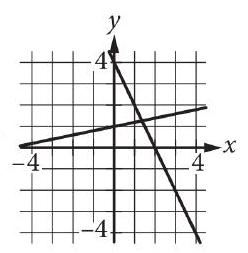
\includegraphics[width=0.23\textwidth]{images/2025_06_15_7d5ca6a095740ea44a32g-15} &
  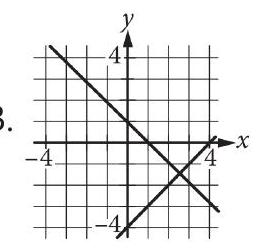
\includegraphics[width=0.23\textwidth]{images/2025_06_15_7d5ca6a095740ea44a32g-15(1)} &
  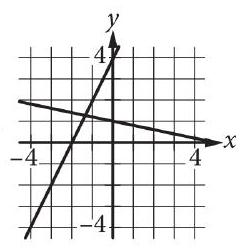
\includegraphics[width=0.23\textwidth]{images/2025_06_15_7d5ca6a095740ea44a32g-15(3)} &
  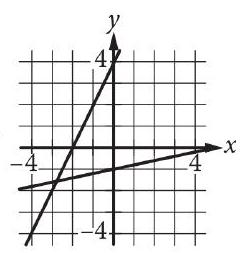
\includegraphics[width=0.23\textwidth]{images/2025_06_15_7d5ca6a095740ea44a32g-15(2)} \\
  \end{tabular}
  \end{center}
  \begin{subanswer}
    % your answer here
  \end{subanswer}

  \item \textbf{System Value} (10 points)\\
  \[\begin{gathered}
  x=10 \\
  y=x+21
  \end{gathered}\]
  The solution to the given system of equations is $(x,y)$. What is the value of $y$?\\
  \begin{enumerate}[label=(\Alph*)]
    \item 2.1
    \item 10
    \item 21
    \item 31
  \end{enumerate}
  \begin{subanswer}
    % your answer here
  \end{subanswer}

  \item \textbf{System Solution} (10 points)\\
  \[\begin{gathered}
  y=-\frac{1}{9}x \\
  y=\frac{1}{2}x
  \end{gathered}\]
  The solution to the given system of equations is $(x,y)$. What is the value of $x$?\\
  \begin{enumerate}[label=(\Alph*)]
    \item -9
    \item -7
    \item 0
    \item 2
  \end{enumerate}
  \begin{subanswer}
    % your answer here
  \end{subanswer}

  \newpage

  \item \textbf{Bus Travel} (10 points)\\
  A bus traveled on the highway and on local roads to complete a trip of 160 miles. The trip took 4 hours. The bus traveled at an average speed of 55 miles per hour (mph) on the highway and an average speed of 25 mph on local roads. If $x$ is the time, in hours, the bus traveled on the highway and $y$ is the time, in hours, it traveled on local roads, which system of equations represents this situation?\\
  \begin{enumerate}[label=(\Alph*)]
    \item $\begin{aligned} 55x+25y&=4 \\ x+y&=160 \end{aligned}$
    \item $\begin{aligned} 55x+25y&=160 \\ x+y&=4 \end{aligned}$
    \item $\begin{aligned} 25x+55y&=4 \\ x+y&=160 \end{aligned}$
    \item $\begin{aligned} 25x+55y&=160 \\ x+y&=4 \end{aligned}$
  \end{enumerate}
  \begin{subanswer}
    % your answer here
  \end{subanswer}

  \item \textbf{System Solution} (10 points)\\
  \[\begin{gathered}
  y=2x+3 \\
  x=1
  \end{gathered}\]
  What is the solution $(x,y)$ to the given system of equations?\\
  \begin{enumerate}[label=(\Alph*)]
    \item $(1,2)$
    \item $(1,5)$
    \item $(2,3)$
    \item $(2,7)$
  \end{enumerate}
  \begin{subanswer}
    % your answer here
  \end{subanswer}

  \newpage

  \item \textbf{System Graph} (10 points)\\
  A system of two linear equations is graphed in the $xy$-plane below.\\
  \insertimage{0.40}{images/2025_06_15_7d5ca6a095740ea44a32g-20}{reference attached}

  Which of the following points is the solution to the system of equations?\\
  \begin{enumerate}[label=(\Alph*)]
    \item $(3,9)$
    \item $(6,15)$
    \item $(8,10)$
    \item $(12,18)$
  \end{enumerate}
  \begin{subanswer}
    % your answer here
  \end{subanswer}
\end{enumerate}